% \begin{titlepage}
%     \begin{center}
%     \vspace*{1cm}

%       \title{Nutrition's Route to Behaviour and Vice Versa:\\ Longitudinal Links from Early Life to Adolescence}
%       \date{}
%       \vfill
%       \author{Yvonne Willemsen}
%       \vfill
%     \end{center}
% \end{titlepage}
\newpage
\thispagestyle{empty}
    \begin{tikzpicture}[remember picture, overlay]
      \node[inner sep=0] at (current page.center) {\includegraphics{Figures/cover_final.pdf}};
    \end{tikzpicture}

\newpage
\thispagestyle{empty}


\begin{titlepage}
   \AddToShipoutPictureBG*{%
  \AtPageLowerLeft{%
    \begin{tikzpicture}[remember picture, overlay]
      \node[inner sep=0] at (current page.center) {\includegraphics[width=\paperwidth, height=\paperheight]{Figures/cover_bg.pdf}};
    \end{tikzpicture}
}
}

\begin{Center}
\vspace{15cm}

{\fontsize{15}{14}\selectfont
\noindent \textbf{Heterogeneity maketh the mind: An exploration of electrical heterogeneity in cortical neurons}\\}

\vfill
Nishant Joshi\\
\end{Center}  


\newpage
\thispagestyle{empty}
\begin{spacing}{1.0}
\begin{figure}[h]
    % \hspace*{2cm} % Adjust the horizontal position of the entire figure
    % \vspace*{-1cm} % Adjust the vertical position of the entire figure
    % \centering
    \begin{subfigure}{0.1\linewidth}
        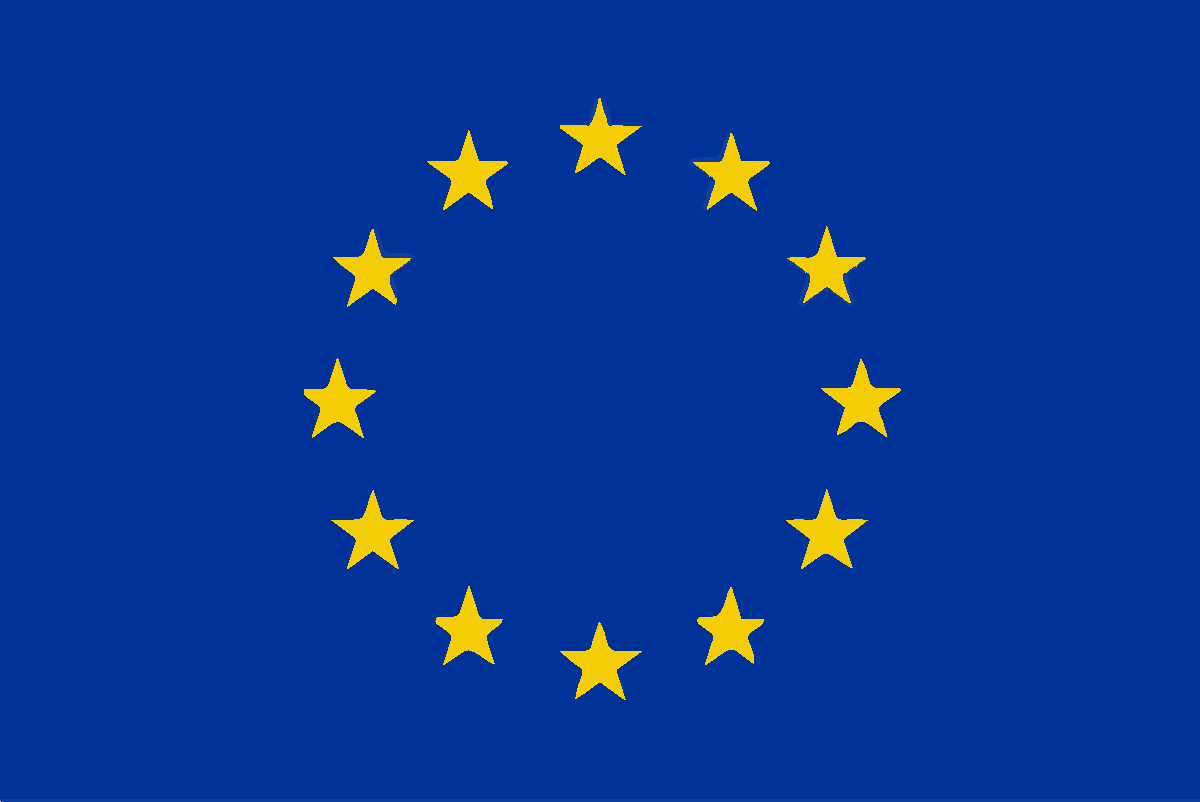
\includegraphics[scale=0.12]{Figures/eu_flag.pdf}
    \end{subfigure}
    \hspace{1.5cm} % Adjust the horizontal space between the images
    \begin{subfigure}{0.1\linewidth}
        
\includegraphics[scale=0.3]{Figures/new-brain-nutrition_logo.pdf}
    \end{subfigure}
\end{figure}

\noindent This project has received funding from the European Union's Horizon 2020 
research and innovation program under the Marie Skłodowska-Curie grant agreement No 860949.
\vspace{0.7cm}

\noindent Author: Nishant Joshi
\newline \noindent Title: Heterogeneity maketh the mind: An exploration of electrical heterogeneity in cortical neurons
\vspace{0.7cm}

\newline \noindent Radboud Dissertations Series
ISSN: 
\vspace{0.7cm}

\newline \noindent Published by RADBOUD UNIVERSITY PRESS 
\newline \noindent Postbus 9100, 6500 HA Nijmegen, The Netherlands 
\newline \noindent www.radbouduniversitypress.nl 
\vspace{0.7cm}

\newline \noindent Design: Nishant Joshi
\newline \noindent Cover: TBD
\newline \noindent Printing: 
\vspace{0.7cm}

\noindent ISBN: 
\newline \noindent DOI: 
\newline \noindent Free download at: www.boekenbestellen.nl/radboud-university-press/dissertations
\vspace{0.7cm}

\newline \noindent © Nishant Joshi, 2025

\begin{figure}[h]

\includegraphics[scale=0.1]{Figures/rup.pdf}
\end{figure}


\begin{justify} 
\noindent This is an Open Access book published under the terms of Creative Commons Attribution-Noncommercial-NoDerivatives International license (CC BY-NC-ND 4.0). This license allows reusers to copy and distribute the material in any medium or format in unadapted form only, for noncommercial purposes only, and only so long as attribution is given to the creator, see http://creativecommons.org/licenses/by-nc-nd/4.0/. 
\end{justify}

\end{spacing}
  
\newpage
\thispagestyle{empty}
  \begin{center}
       \vspace*{0cm}
        
       \textbf{\Large Heterogeneity maketh the mind: An exploration of electrical heterogeneity in cortical neurons}\\
          
       \vspace{2cm}

       Proefschrift ter verkrijging van de graad van doctor\\
        aan de Radboud Universiteit Nijmegen \\
        op gezag van de rector magnificus prof. dr. J.M. Sanders,\\
        volgens besluit van het college voor promoties\\
        in het openbaar te verdedigen op\\

        \vspace{1cm}
        % maandag 15 april 2024\\
        % om 16:30 uur precies\\
        \vspace{1cm}
        door\\

        \vspace{1cm}
        
        Nishant Joshi\\
        geboren op 26 January 1994\\
        te Varanasi, India\\
       \vfill
     
       % \includegraphics[width=0.4\textwidth]{university}
            
       % Department Name\\
       % University Name\\
       % Country\\
       % Date
            
   \end{center}  
\end{titlepage}


\newpage
\thispagestyle{empty}
\noindent{\textbf{Promotor:}}
\newline{Prof. dr. T. Celikel}
\vspace{1cm}
\newline{\textbf{Copromotoren:}}
\newline{Dr. F. Zeldenrust}
\vspace{1cm}
\newline{\textbf{Manuscriptcommissie:}}
\newline{TBD.}
\newline{TBD.}
\newline{TBD.}
\newline{TBD.}
\newline{TBD.}

\newpage
\thispagestyle{empty}
\noindent{\textbf{Funding}} 
\newline{This project has received funding from the European Union's Horizon 2020 research and innovation program under the Marie Skłodowska-Curie grant agreement No 860949.}


\newpage\null\thispagestyle{empty}\newpage